\chapter{Release 1}
\section{Introduction}


Le terme release d\'{e}signe ici une version de notre application constitu\'{e}e d'une suite d'it\'{e}rations
qui se terminent quand les incr\'{e}ments de ces derniers construisent un produit pr\'{e}sentant
suffisamment de valeur \`{a} l'utilisateur.

Dans ce chapitre, nous nous intéressons principalement par l'application web ,et nous allons nous int\'{e}resser \`{a} la premi\`{e}re release dans laquelle nous traitons en d\'{e}tails chacun des cas d'utilisation pr\'{e}alablement pr\'{e}sent\'{e}s.
Ainsi ,selon le sprint ,on précisons l'analyse qui consiste  \`{a} illustrer le diagramme de cas d'utilisation ,la conception pour pr\'{e}senter
le diagramme de s\'{e}quence et le sch\'{e}ma  de base de donn\'{e}es et nous finissons par le test en pr\'{e}sentant
les interfaces correspondantes.

Pour chaque sprint on va pr\'{e}senter le cas d'utilisation,la conception
qui consistre à pr\'{e}senter le diagramme de  s\'{e}quence
et nous finissons par l'illustration du sch\'{e}ma de la base de donn\'{e}es  des modules correspondants.

Ainsi ,contrairement aux cycles de d\'{e}veloppement s\'{e}quentiel, avec la m\'{e}thodologie agile, le test n'est
pas une phase qui se d\'{e}roule apr\`{e}s la fin de d\'{e}veloppement. En effet, les tests seront int\'{e}gr\'{e}s
d\`{e}s le d\'{e}but du premier sprint jusqu'\`{a} la livraison du produit final.

Enfin ,nous illustrons  la m\'{e}thode de liason de donn\'{e}es que nous avons suivi
ainsi nous présentons le diagramme de classes ,le diagramme  d'activit\'{e} et le diagramme  de d\'{e}ploiement
pour mieux expliquer notre application.


\section{ Sprint 1 }


\subsection{Analyse}

    \textbf{ Diagramme de cas d'utilisation "G\'{e}rer un membre"}
    \begin{figure}[H]
    \center
    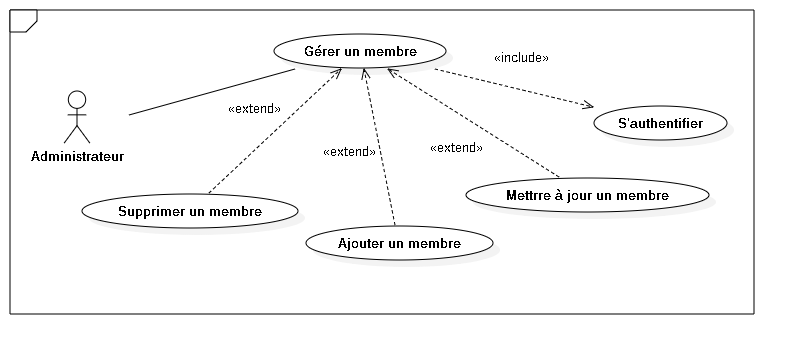
\includegraphics[width=13cm,height=8cm]{./figures/ucM.png}
    \caption{G\'{e}rer un membre.}

    \end{figure}

\subsection{Conception}

Le diagramme de s\'{e}quence indique l'interaction entre plusieurs acteurs
afin d'expliquer le d\'{e}roulement des diff\'{e}rents sc\'{e}nario entre les diff\'{e}rents
\'{e}l\'{e}ments du projet.

\subsubsection{Le sc\'{e}nario \guillemotleft{} Cr\'{e}ation d'un membre \guillemotright{}}

Le diagramme de s\'{e}quence \guillemotleft{} Ajout d'une t\^{a}che \guillemotright{} pr\'{e}sente le s\'{e}quencement
des interactions entre Administrateur, Application et Base de donn\'{e}es (BD).

\newpage
\subsection{Sch\'{e}ma}

\textbf{La table \guillemotleft{} members \guillemotright{}}

\begin{table}

\begin{tabular}{|l|l|l|l|l|l|}
\hline
Field        & Type         & Null & Key & Default            & Extra            \\
\hline
id           & int(11)      & NO   & PRI & NULL               & auto\_increment  \\
\hline
login        & varchar(30)  & YES  &     & NULL               &                  \\
\hline
password     & varchar(15)  & YES  &     & NULL               &                  \\
\hline
firstname    & varchar(50)  & YES  &     & NULL               &                  \\
\hline
lastname     & varchar(30)  & YES  &     & NULL               &                  \\
\hline
email        & varchar(100) & YES  &     & NULL               &                  \\
\hline
hiredate     & datetime     & YES  &     & CURRENT\_TIMESTAMP &                  \\
\hline
color        & varchar(6)   & YES  &     & NULL               &                  \\
\hline
projects\_id & int(11)      & YES  & MUL & NULL               &                  \\
\hline
pname        & varchar(50)  & YES  &     & NULL               &                  \\
\hline
\end{tabular}
\centering
 \caption {Members.}
\end{table}


\subsection{Test}

Dans ce premier sprint, nous testons la fonctionnalit\'{e}
« Gestion des membres» qui affiche, ajoute,
supprime les membres de la base de donn\'{e}es.
Ci-dessus nous ajoutons des captures \'{e}cran du sprint r\'{e}alis\'{e}.

\bigskip
\bigskip

Lors de la cr\'{e}ation d'un utilisateur , un email contenant son mot de passe lui
sera envoy\'{e}, ainsi si on modifie les param\'{e}tres d'utilisateur , un nouveeau
mot de passe lui sera envoy\'{e} sur la nouvelle addresse email .

\bigskip
\bigskip

\begin{figure}[H]
\center
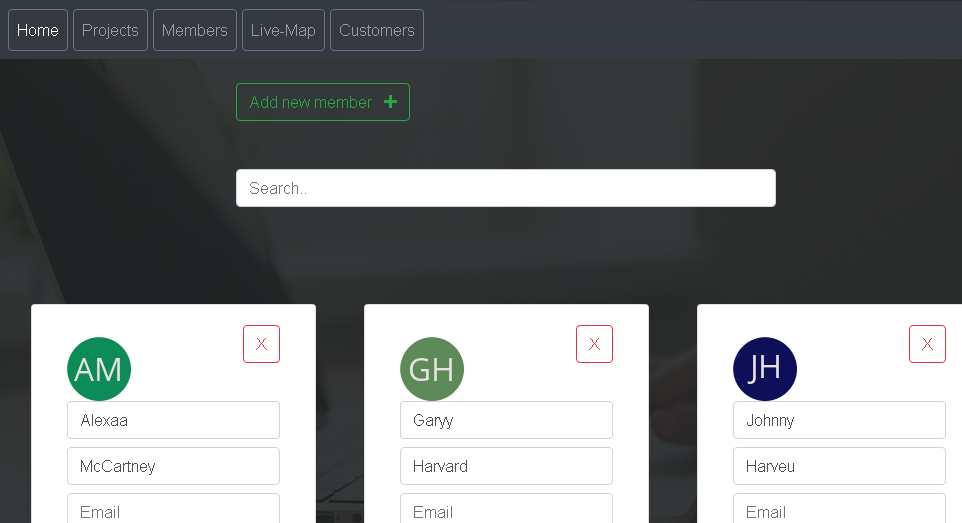
\includegraphics[width=11cm,height=7cm]{./figures/pres/mm1.png}
\caption{Gestion des membres.1.}
\end{figure}

\begin{figure}[H]
\center
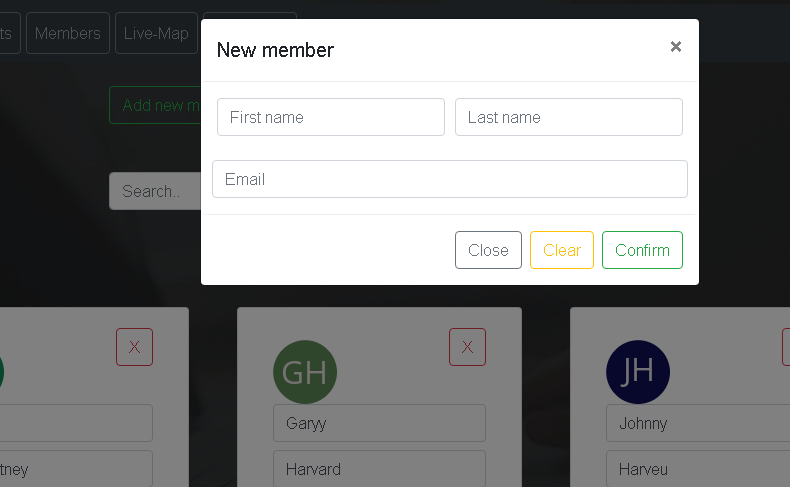
\includegraphics[width=11cm,height=7cm]{./figures/pres/mm2.png}
\caption{Gestion des membres.2.}
\end{figure}




\begin{figure}[H]
\center
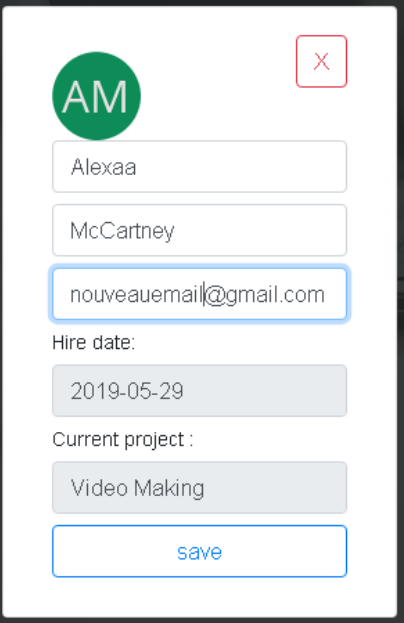
\includegraphics[width=11cm,height=7cm]{./figures/pres/mm3.png}
\caption{Gestion des membres.3.}
\end{figure}




\section{ Sprint 2 }
%clients

\subsection{Analyse}
\subsubsection{ Diagramme de cas d'utilisation "G\'{e}rer un client"}
\begin{figure}[H]
\center
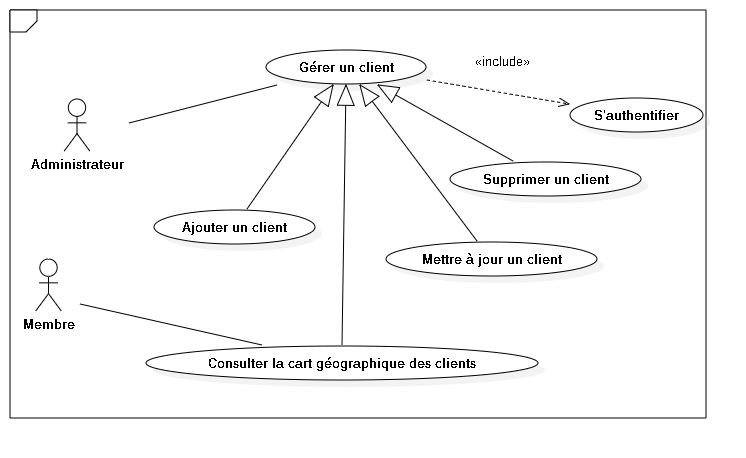
\includegraphics[width=13cm,height=8cm]{./figures/ucC.png}
\caption{G\'{e}rer un client.}
\end{figure}

\subsection{Conception}
\subsubsection{Le sc\'{e}nario \guillemotleft{} Cr\'{e}ation d'un client\guillemotright{}}
Le diagramme de s\'{e}quence \guillemotleft{} Ajout d'une t\^{a}che \guillemotright{} pr\'{e}sente le s\'{e}quencement
des interactions entre Administrateur, Application et Base de donn\'{e}es (BD).

\begin{figure}[H]
\center
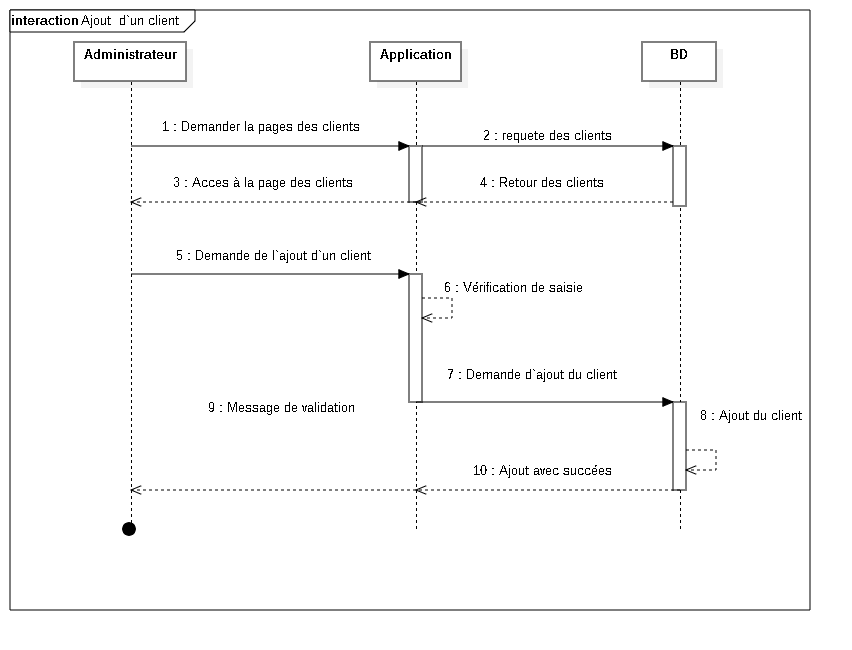
\includegraphics[width=14cm,height=9cm]{./figures/seq/F.png}
\caption{Cr\'{e}ation d'une client.}
\end{figure}



\subsubsection{Le sc\'{e}nario \guillemotleft{} Consultation de la carte g\'{e}ographique des clients\guillemotright{}}
Le diagramme de s\'{e}quence \guillemotleft{} Ajout d'une t\^{a}che \guillemotright{} pr\'{e}sente le s\'{e}quencement
des interactions entre Administrateur, Application et Base de donn\'{e}es (BD).



\subsubsection{Sch\'{e}ma}
\textbf{ La table \guillemotleft{} customers \guillemotright{}}


\begin{table}

\begin{tabular}{|l|l|l|l|l|l|}
\hline
Field            & Type          & Null & Key & Default            & Extra            \\
\hline
id               & int(11)       & NO   & PRI & NULL               & auto\_increment  \\
\hline
name             & varchar(45)   & YES  &     & NULL               &                  \\
\hline
phone            & varchar(45)   & YES  &     & NULL               &                  \\
\hline
address          & varchar(1000) & YES  &     & NULL               &                  \\
\hline
email            & varchar(50)   & YES  &     & NULL               &                  \\
\hline
longitude        & double        & YES  &     & NULL               &                  \\
\hline
latitude         & double        & YES  &     & NULL               &                  \\
\hline
subscriptionDate & datetime      & YES  &     & CURRENT\_TIMESTAMP &                  \\
\hline
\end{tabular}
\centering
\caption{Customers}
\end{table}


\subsection{Test}

\FloatBarrier
\begin{figure}[H]
\center
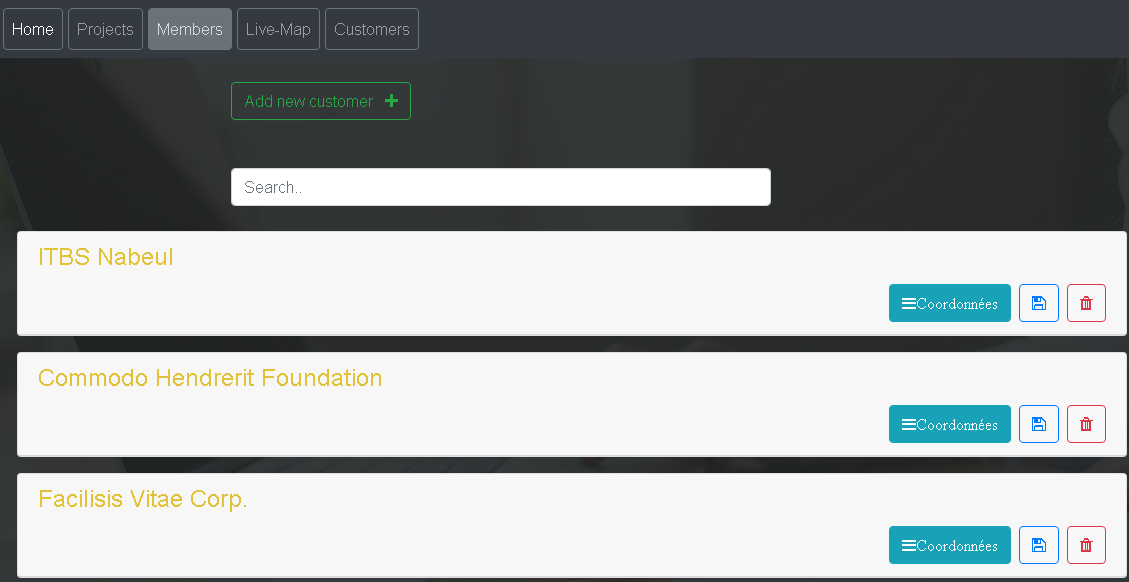
\includegraphics[width=11cm,height=7cm]{./figures/pres/cc1.png}
\caption{Gestion des clients.1.}
\end{figure}
\FloatBarrier


\FloatBarrier
\begin{figure}[H]
\center
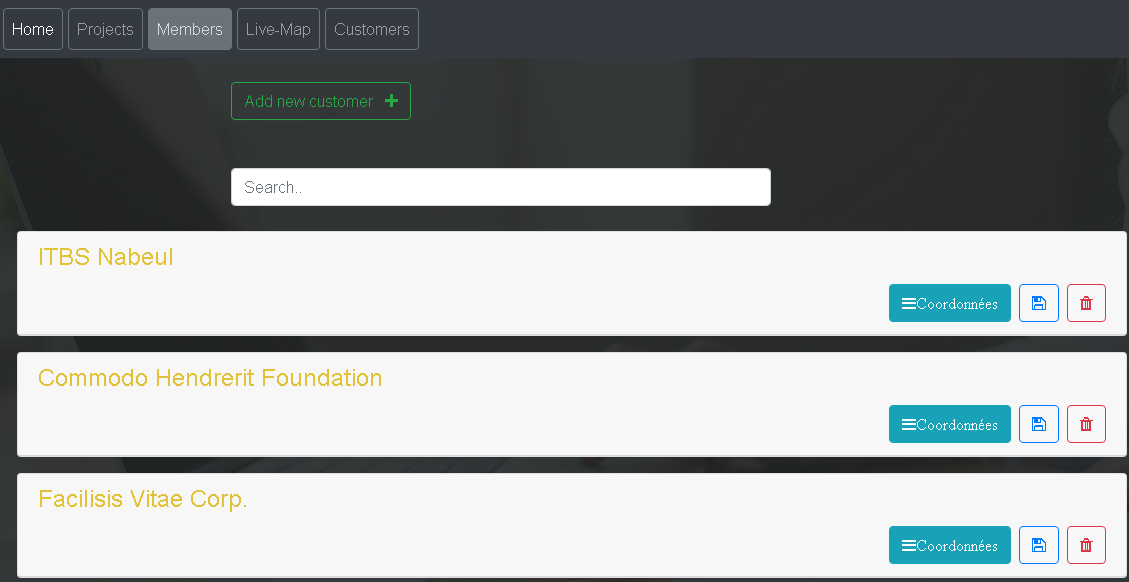
\includegraphics[width=11cm,height=7cm]{./figures/pres/cc1.png}
\caption{Gestion des clients.2.}
\end{figure}
\FloatBarrier
\subsection{Consultation carte g\'{e}ographique des clients}

\FloatBarrier
\begin{figure}[H]
\center
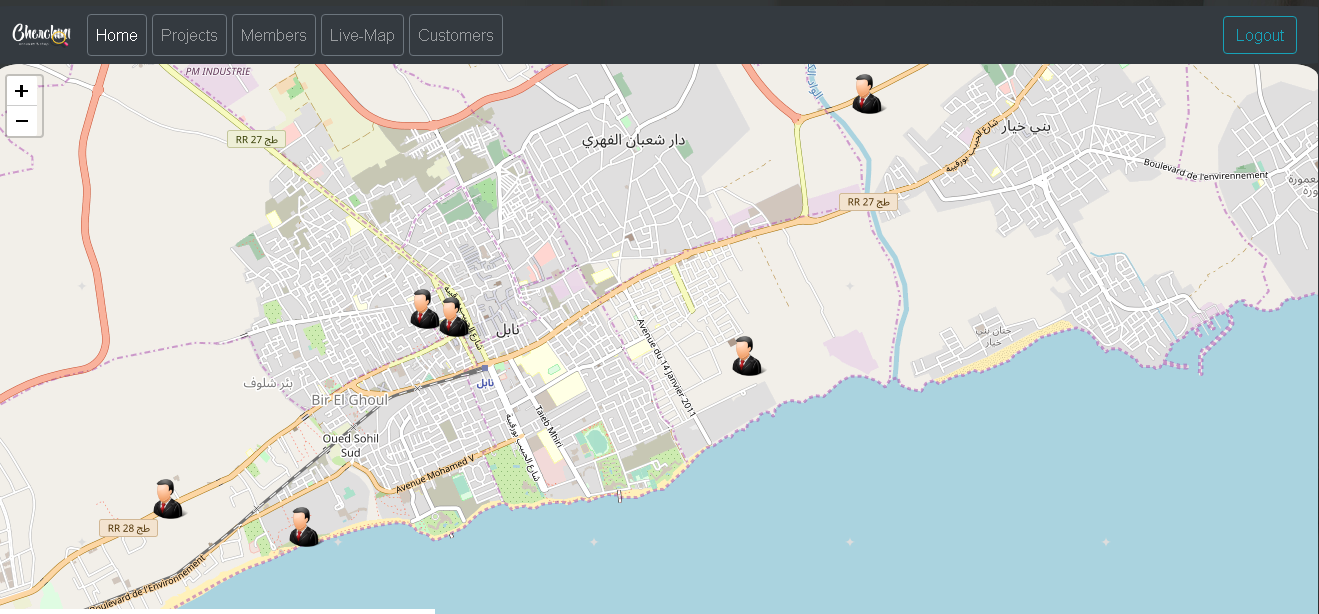
\includegraphics[width=15cm,height=10cm]{./figures/pres/map.png}
\caption{Carte g\'{e}ographique.}
\end{figure}
\FloatBarrier


\section{ Sprint 3 }
\subsubsection{Analyse}
\subsubsection{Conception}
\subsubsection{Code}
\subsubsection{Test}

\section{ Sprint 4 }
%auth

\subsection{Conception}
\textbf{Le sc\'{e}nario \guillemotleft{} Authentification \guillemotright{}}

Ce sch\'{e}ma pr\'{e}sente le m\^{e}me sc\'{e}nario pour l'administrateur et un simple
membre.(Figure 3.20) et (Figure 3.21)

\begin{figure}[H]
\center
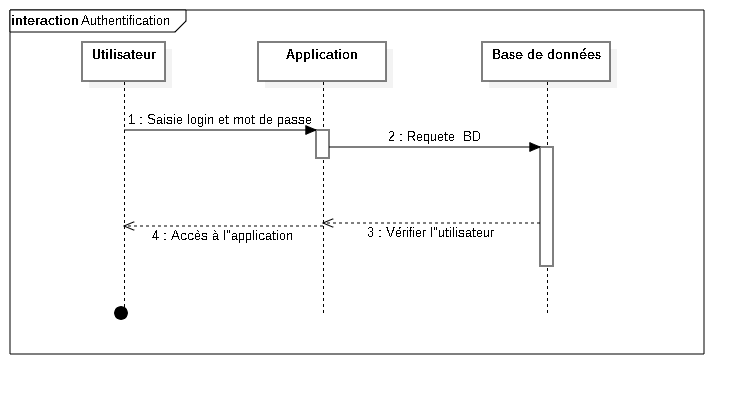
\includegraphics[width=14cm,height=8cm]{./figures/seq/A.png}
\caption{Authentification.}
\end{figure}


\subsection{Test}


\begin{figure}[H]
\center

\includegraphics[width=11cm,height=7cm]{./figures/pres/1.png}
\caption{Accueil.}

\end{figure}


\section{Structure de l'application}
Le sh\'{e}ma suivant pr\'{e}sente la structure de notre application


\begin{figure}[H]
\center
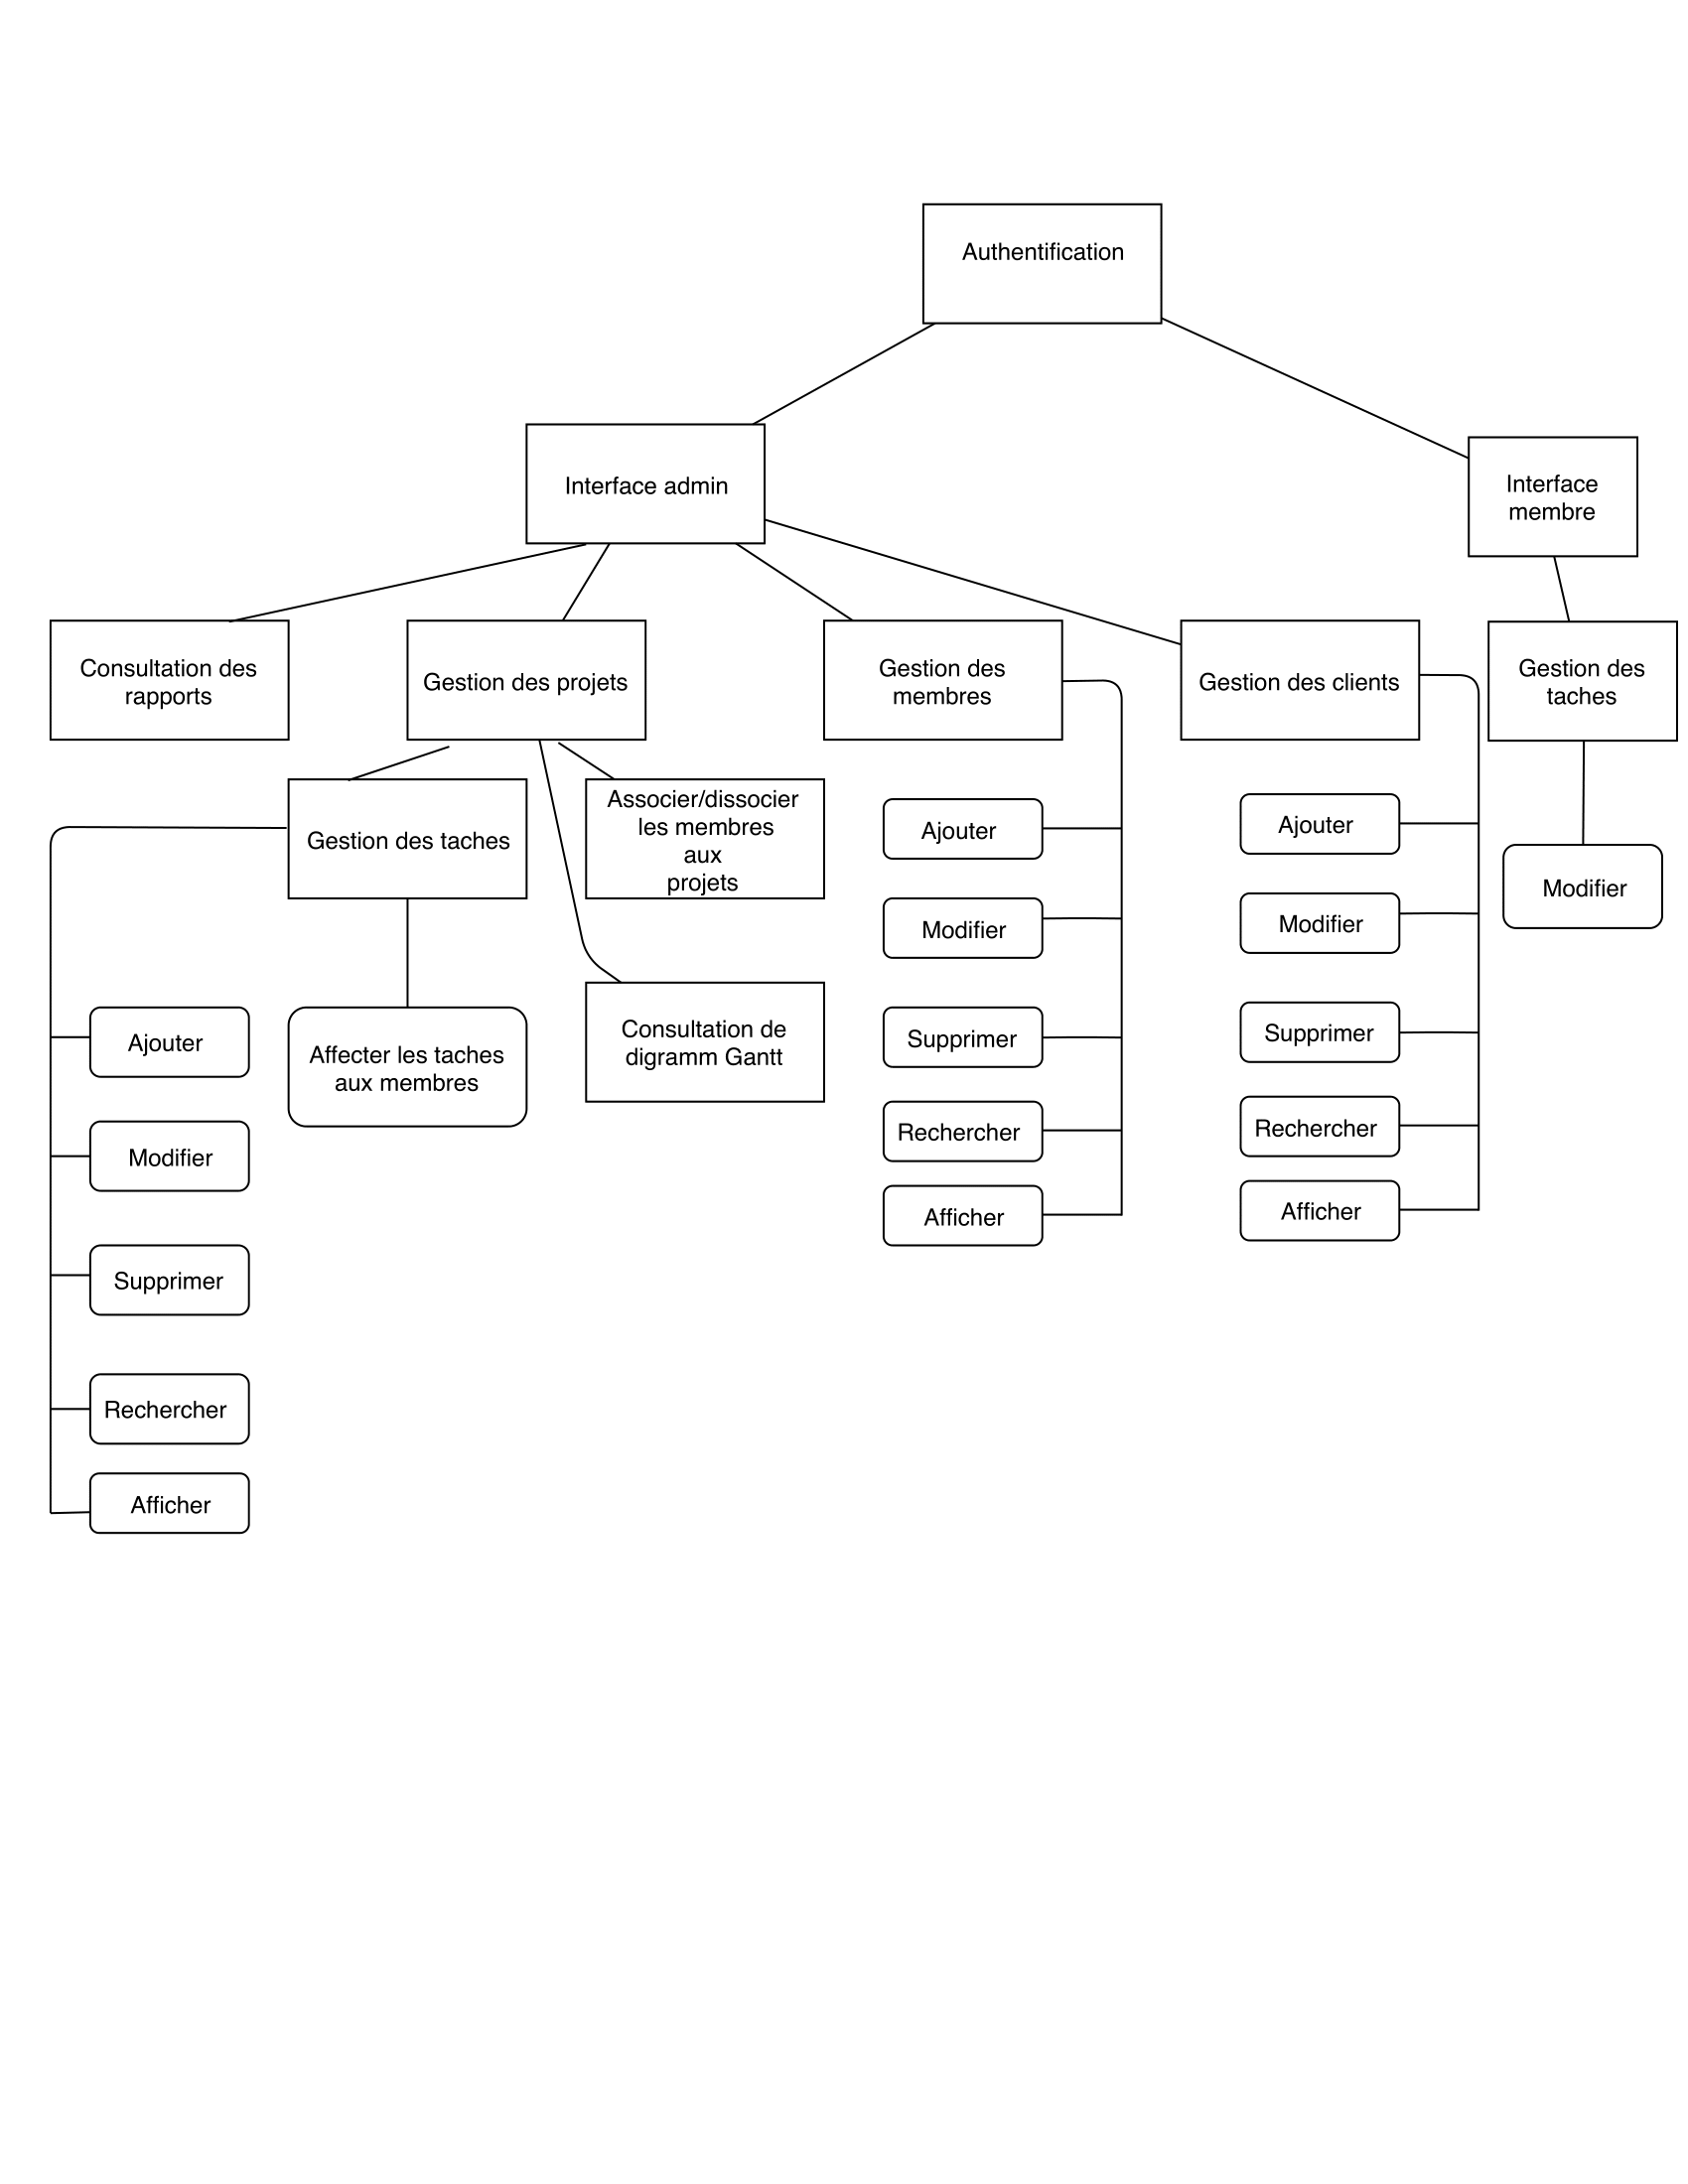
\includegraphics[width=13cm,height=15cm]{./figures/structure.png}
\caption{Structure de l'application web.}
\end{figure}


\section{Conception de la base de donn\'{e}es}

\subsection{Mod\`{e}le du liason des donn\'{e}es }
L'architecture de notre application nous implique \`{a} cr\'{e}er un mod\`{e}le physique
des donn\'{e}es , et nous avons pas \'{e}t\'{e} besoin d'un model conceptuel logique
,puisque on a li\'{e}e directement les donn\'{e}es \`{a} l'application par le biais d'un
pilote de connexion et pas par un ORM , et ceci est le diagramme
Entit\'{e}s \textendash{}Relations de la base de donn\'{e}es qui est en interaction avec
l'application web .
Choix de la m\'{e}thodologie de conception :
La liaison par des ORM ,ou poss\'{e}de des avantages bienque des inconv\'{e}nient ,
parmi ses avantages :

\bigskip
\begin{itemize}
\item{\textbf{La portabilit\'{e} :}  ORM est utilis\'{e} pour que vous \'{e}criviez votre structure une
seule fois et la couche ORM g\'{e}rera l'instruction finale adapt\'{e}e au SGBD
configur\'{e}. C'est un excellent avantage, car une op\'{e}ration simple, telle que
limit, est ajout\'{e}e sous la forme "limit 0,100" \`{a} la fin de l'instruction select
dans MySQL, alors qu'elle est "select top 100 from table" dans MS SQL.}

\bigskip
\item{\textbf{Imbrication de donn\'{e}es:} en cas de relations, la couche ORM extraira
automatiquement les donn\'{e}es pour vous.}

\bigskip
\item{\textbf{Langage unique:} vous ne connaissez pas le langage SQL pour traiter la base
de donn\'{e}es uniquement avec votre langage de d\'{e}veloppement.
Ajouter revient \`{a} modifier: la plupart des couches ORM traitent l'ajout de
nouvelles donn\'{e}es (insertion SQL) et la mise \`{a} jour des donn\'{e}es (SQL
Update) de la m\^{e}me mani\`{e}re, ce qui facilite grandement l'\'{e}criture et la
maintenance du code.}

\item{\textbf{Imbrication de donn\'{e}es:} en cas de relations, la couche ORM extraira
automatiquement les donn\'{e}es pour vous.}

\end{itemize}

\bigskip

Et parmi les inconv\'{e}nients de l'ORM on trouve :



\bigskip

\begin{itemize}
\item{\textbf{ La complexit\'{e} des requ\^{e}tes : }certaines couches ORM ont des limitations, en
particulier lors de l'ex\'{e}cution de requ\^{e}tes. Vous serez donc parfois oblig\'{e}
d'\'{e}crire en SQL brut.}

\item{\textbf{Lenteur:}
 si vous comparez les performances entre l'\'{e}criture de SQL brut ou
l'utilisation d'ORM, vous trouverez le brut beaucoup plus rapidement car il
n'y a pas de couche de traduction.}

\item{\textbf{R\'{e}glage:} si vous connaissez bien le langage SQL et votre SGBD par d\'{e}faut,
vous pouvez utiliser vos connaissances pour acc\'{e}l\'{e}rer les requ\^{e}tes, mais ce
n'est pas la m\^{e}me chose avec ORM.}

\item{\textbf{Configuration:}
 si vous travaillez dans un projet Big Data et que vous n'\^{e}tes
pas satisfait de la performance, vous vous retrouverez en train d'\'{e}tudier la
couche ORM afin de pouvoir minimiser les occurrences du SGBD.}



\end{itemize}


\subsection{Diagramme de classes}

\begin{figure}[H]
\center
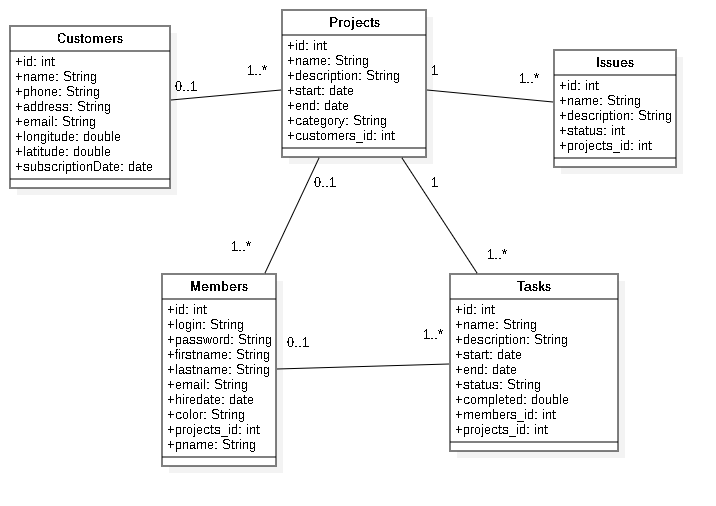
\includegraphics[width=13cm,height=11cm]{./figures/class.png}
\caption{Diagramme de classes.}

\end{figure}


\subsubsection{Tableau explicatif}



\begin{table}

\begin{tabular}{|l|l|l|l|l|}
\hline
Nom relation                        & Entité E1                 & Entité E2                  & Relation(E1:E2) & Relation(E2:E1)  \\
\hline
\multirow{2}{*}{Projects -Tasks}    & \multirow{2}{*}{Projects} & \multirow{2}{*}{Tasks}     & 1 : N           & 1 : 1            \\
\cline{4-5}
                                    &                           &                            & Non-identifiée  & identifiée       \\
\hline
\multirow{2}{*}{Projects -Members}  & \multirow{2}{*}{Projects} & \multirow{2}{*}{Members}   & 1~: N           & 1~: 1            \\
\cline{4-5}
                                    &                           &                            & Non-identifiée  & Non-identifiée   \\
\hline
\multirow{2}{*}{Members-Tasks}      & \multirow{2}{*}{Members}  & \multirow{2}{*}{Tasks}     & 1~: N           & 1~: 1            \\
\cline{4-5}
                                    &                           &                            & Non-identifiée  & Non-identifiée   \\
\hline
\multirow{2}{*}{Projects-Customers} & \multirow{2}{*}{Projects} & \multirow{2}{*}{Customers} & 1~: 1           & 1~: N            \\
\cline{4-5}
                                    &                           &                            & Non-identifiée  & Non-identifiée   \\
\hline
\end{tabular}
\centering
\caption {Relations}
\end{table}


\newpage



\section{Diagramme de d\'{e}ploiement }
\subsection{Diagramme de d\'{e}ploiement}


\begin{itemize}
\item{ \textbf{Le Client :} C'est le navigateur web, il permet aux utilisateurs d'acc\'{e}der au
serveur, c'est d'interface \`{a} l'utilisateur.}

\item{ \textbf{Le serveur web :} C'est le serveur principal qui abrite les diff\'{e}rents composants logiciels de
notre application. Il assure la gestion des connexions et des requ\^{e}tes du client
ainsi que aussi la distribution et rendu (rendering) des pages EJS.
Cet \'{e}l\'{e}ment contient principalement un environnement d'ex\'{e}cution qui est
le framework javascript Node js sur lequel est d\'{e}ploy\'{e} l'application
Web(Express JS ).}

\item{ \textbf{La base de donn\'{e}es :} Est exploit\'{e} par le avec le serveur wamp.
C'est le composant qui s'occupe du stockage et de la gestion des donn\'{e}es.
La communication des donn\'{e}es entre l'application est la base de donn\'{e}es
est assur\'{e}e par le pilote ( driver ) de mysql pour Node js.}


\end{itemize}





\begin{figure}[H]
\center
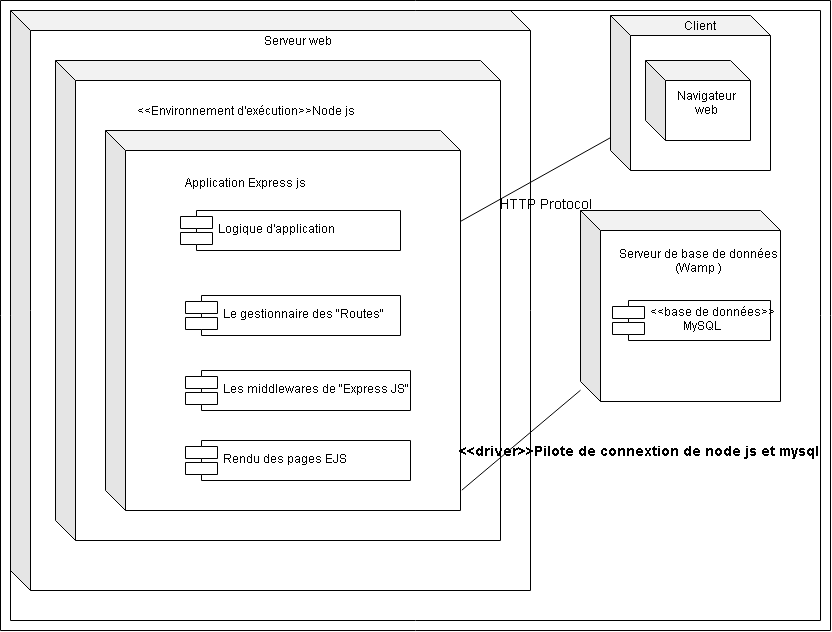
\includegraphics[width=13cm,height=11cm]{./figures/deployement.png}
\caption{Diagramme de d\'{e}ploiement.}
\end{figure}
\FloatBarrier


\newpage

\section{Diagramme d'activit\'{e}}
Le diagramme d'activit\'{e} nous permet de d\'{e}crire les traitements. Il est
particuli\`{e}rement adapt\'{e} \`{a} la mod\'{e}lisation du cheminement de flots de
contr\^{o}le et de flots de donn\'{e}es. Il permet ainsi de repr\'{e}senter le
comportement d'une m\'{e}thode ou le d\'{e}roulement d'un cas d'utilisation dans
un graphe.
Les diagrammes d'activit\'{e}s sont tr\`{e}s proches des diagrammes d'\'{e}tats-
transitions dans leur pr\'{e}sentation, mais leur interpr\'{e}tation est diff\'{e}rente.
Une activit\'{e} repr\'{e}sente une ex\'{e}cution d'un m\'{e}canisme, un d\'{e}roulement
d'\'{e}tapes s\'{e}quentielles. Le passage d'une activit\'{e} vers une autre est mat\'{e}rialis\'{e}
par une transition.
Les transitions sont d\'{e}clench\'{e}es par la fin d'une activit\'{e} et provoquent le
d\'{e}but imm\'{e}diat d'une autre.
Dans la page suivante , nous pr\'{e}sentons notre diagramme d'activit\'{e} qui illustre le
d\'{e}roulement s\'{e}quentiel des traitements accomplis par l'administrateur afin de
cr\'{e}er et g\'{e}rer un projet.
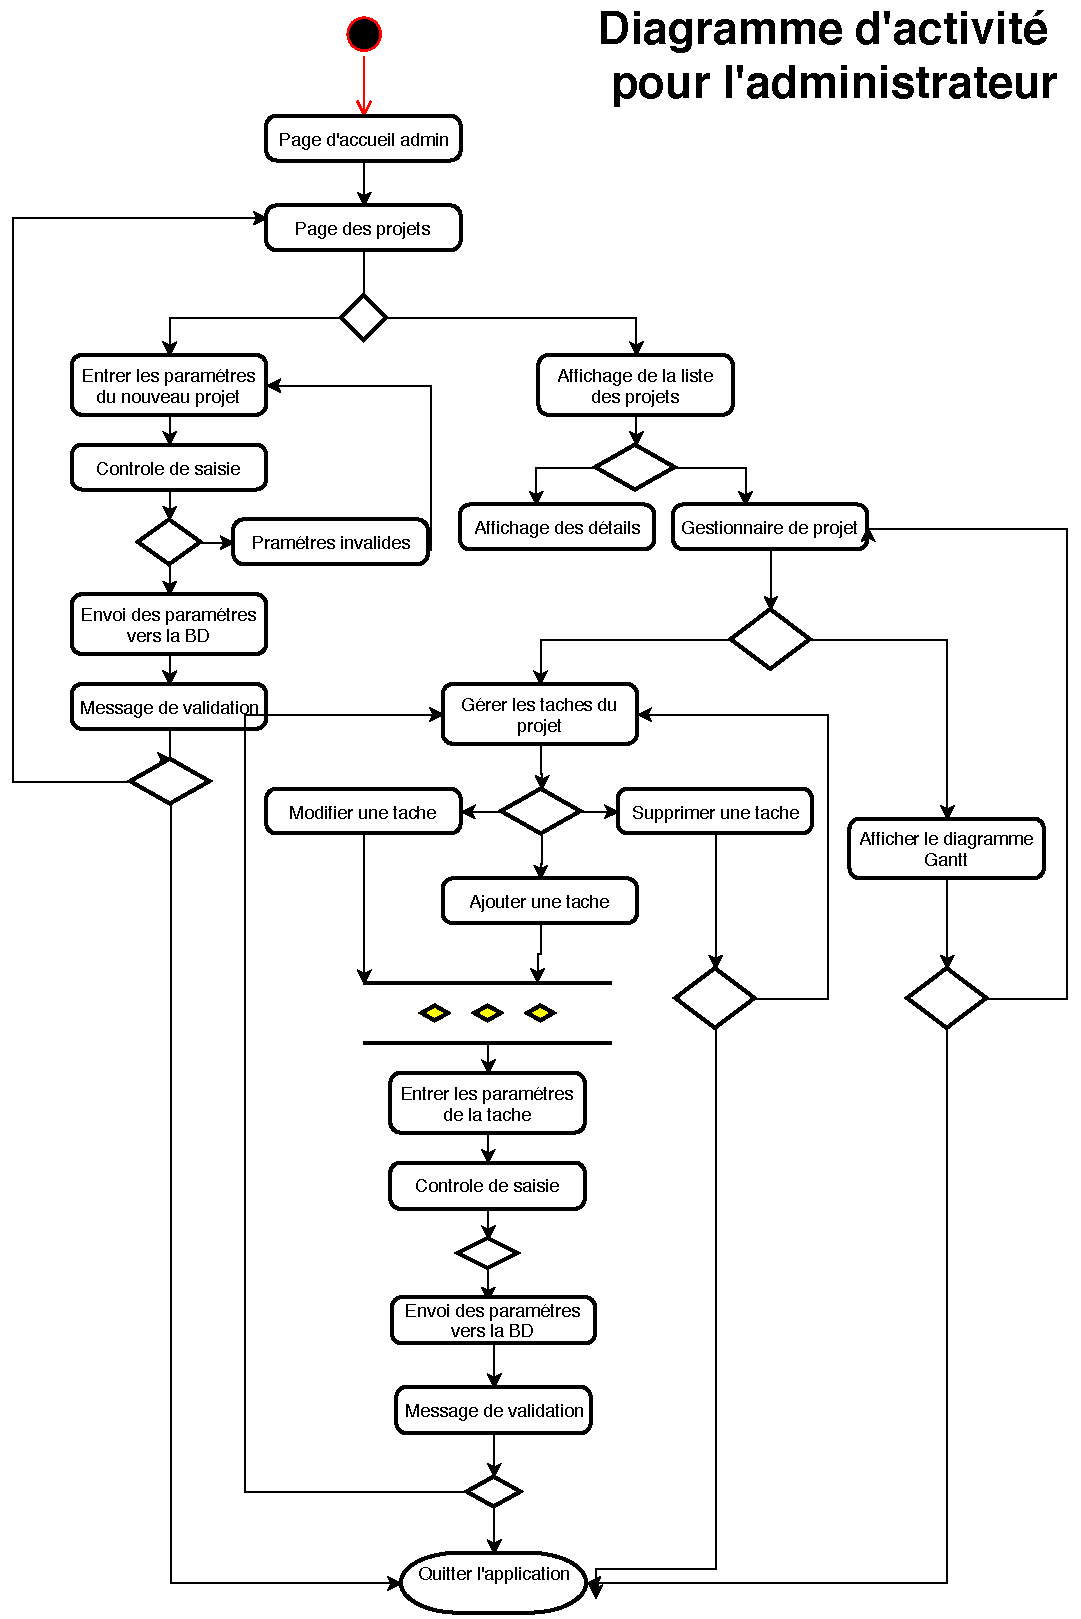
\includepdf{./pdf/activity.pdf}


Ainsi , la figure suivante représente le diagramme d'activit\'{e} pour un membre :
\begin{figure}[H]
\center
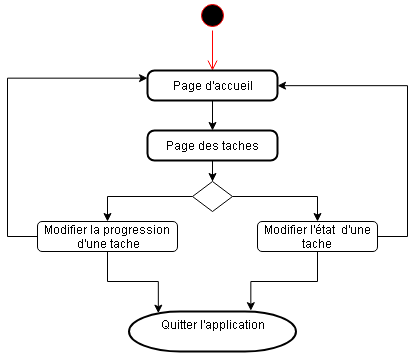
\includegraphics[width=13cm,height=11cm]{./figures/activity_m.png}
\caption{Diagramme d'activit\'{e} pour un membre.}

\end{figure}




